\documentclass[12pt,letterpaper]{article}
\usepackage{fullpage}
\usepackage[top=2cm, bottom=4.5cm, left=2.5cm, right=2.5cm]{geometry}
\usepackage{amsmath,amsthm,amsfonts,amssymb,amscd}
\usepackage{lastpage}
\usepackage{enumerate}
\usepackage{fancyhdr}
\usepackage{mathrsfs}
\usepackage{xcolor}
\usepackage{graphicx}
\usepackage{listings}
\usepackage{hyperref}
\usepackage{tikz-qtree}

\hypersetup{%
  colorlinks=true,
  linkcolor=blue,
  linkbordercolor={0 0 1}
}
 
\renewcommand\lstlistingname{Algorithm}
\renewcommand\lstlistlistingname{Algorithms}
\def\lstlistingautorefname{Alg.}

\lstdefinestyle{Python}{
    language        = Python,
    frame           = lines, 
    basicstyle      = \footnotesize,
    keywordstyle    = \color{blue},
    stringstyle     = \color{green},
    commentstyle    = \color{red}\ttfamily
}

\setlength{\parindent}{0.0in}
\setlength{\parskip}{0.05in}
% Edit these as appropriate
\newcommand\course{CSE 3500}
\newcommand\hwnumber{4}                  % <-- homework number
\newcommand\release{}    % <-- release date
\newcommand\due{}        % <-- homework number

\pagestyle{fancyplain}
\headheight 35pt
\lhead{\course}
\chead{\textbf{\Large Homework \hwnumber}}
\rhead{Released on \release \\ Due on \due}
\lfoot{}
\cfoot{}
\rfoot{\small\thepage}
\headsep 1.5em

\begin{document}

\begin{center}
    \LARGE Suffix Trees, Hashing
\end{center}


\section*{Problem 0 -- Suffix Trees on multiple strings (25\%)}
A suffix tree of $m$ strings $(S_1,S_2,\dots,S_m)$ is a suffix tree built from inserting the strings in order: $S_1\$_1$, $S_2\$_2$, $\dots$, $S_m\$_m$ where $\$_1,\dots,\$_m$ are distinct terminating strings.

\begin{figure}[h!]
    \centering
    % \includegraphics[width=0.8\textwidth]{prob_port.png}
    \caption{A suffix tree built for strings PROBABILITY\# and PORTABILITY\$ where \# and \$ are the terminating characters.}
    \label{st}
\end{figure}

\begin{itemize}
    \item Build the suffix tree for BANDANNA\# and SAVANNAH\$.
    \item Give an algorithm to find the longest common substring of $m$ strings, $S_1,\dots,S_m$ using suffix trees. 
    \item What is your algorithms runtime? Show your work/give an argument.
    \item Using your algorithm, what is the longest common substring of BANDANNA\# and SAVANNAH\$?
\end{itemize}    

\begin{enumerate}
    \item 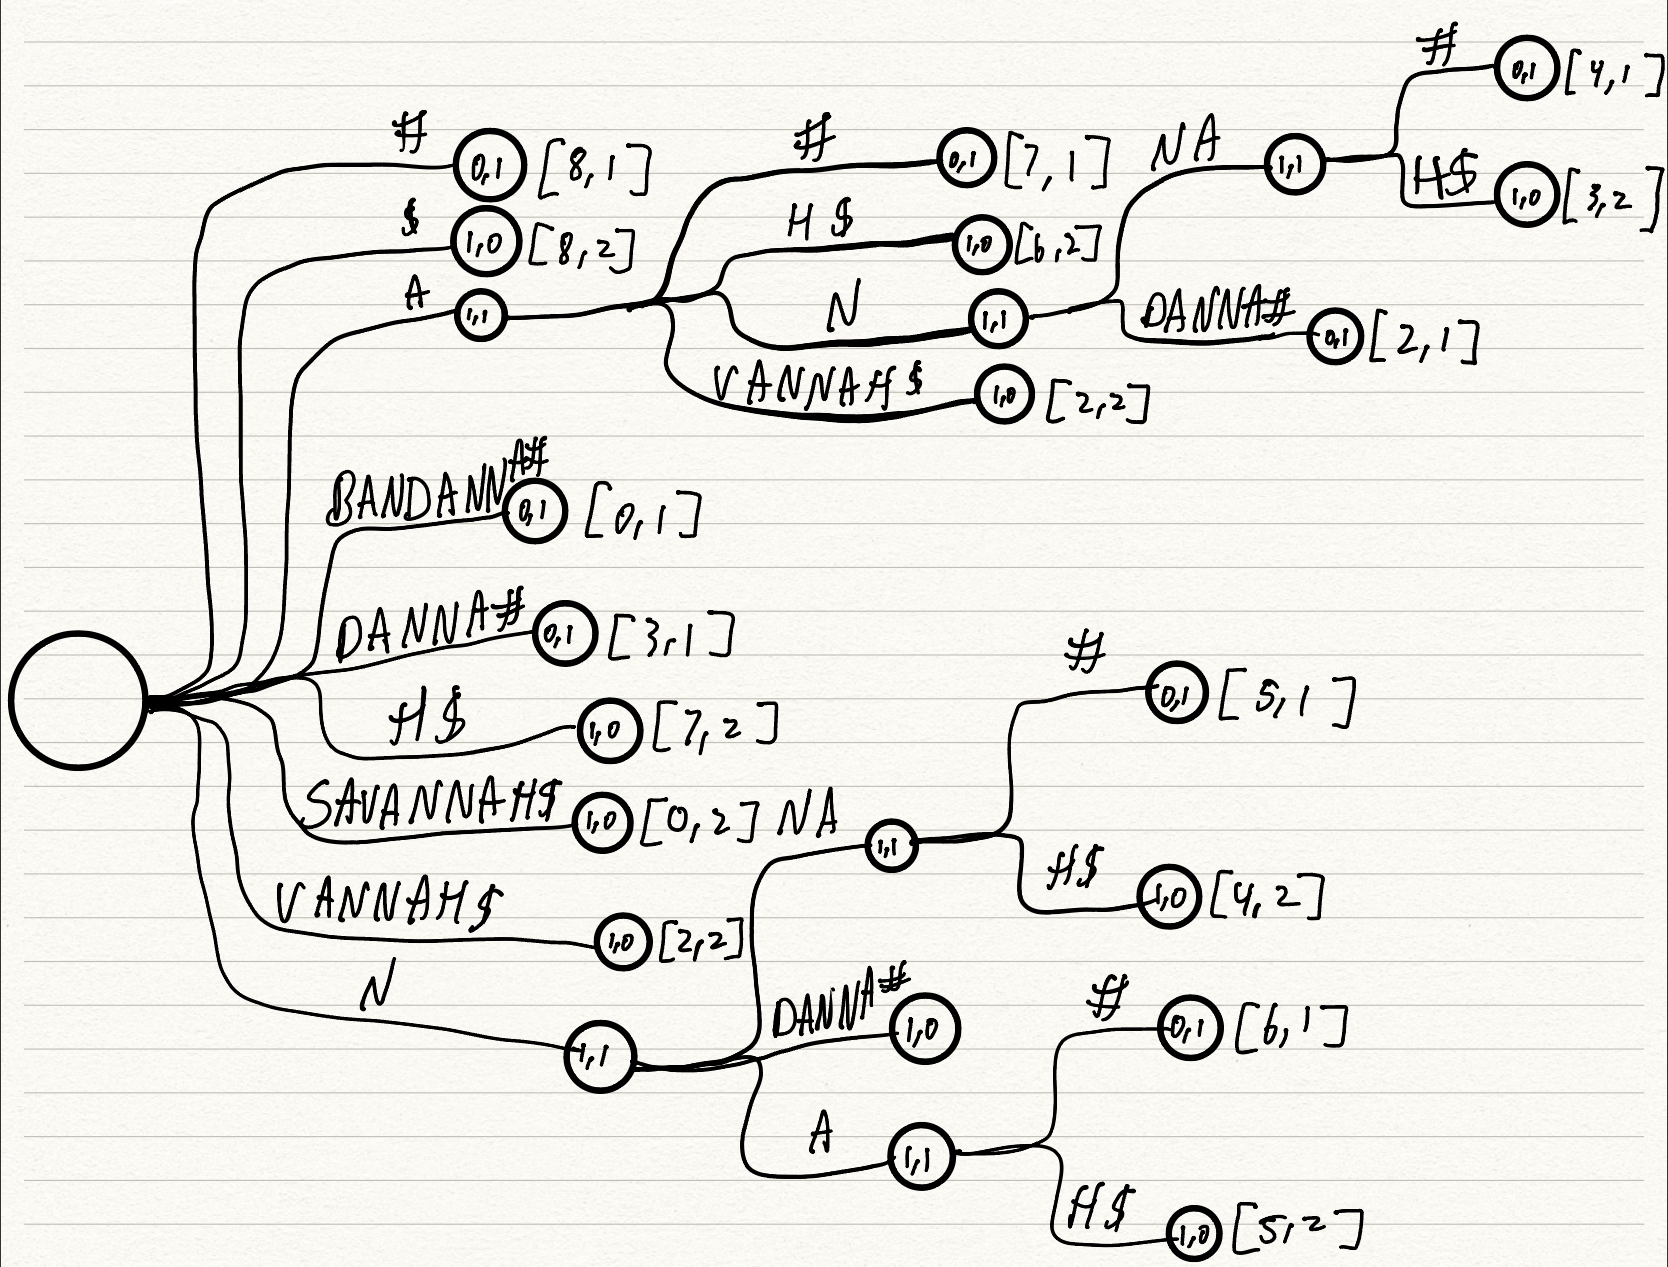
\includegraphics[scale=.2]{./images/Suffixtree-1.png}
    
    (Savannah\$, Bandanna\#) indexes 0 to 8
    \item We can use the suffix tree to find the longest common substring of $m$ strings. 
    We first build a generalized suffix tree for $m$ strings with the edges being the suffixes and the nodes hold the original strings that the suffixes are from.
    We can then find the deepest node in the suffix tree that has children for all $m$ strings. 
    This node will be the deepest subtree in the suffix tree that has a substring that is common to all $m$ strings.
    A algorithm we can use to find the deepest subtree is to do a depth first search on the suffix tree.
    We can use depth first search because we know that the deepest subtree will be the longest path in the suffix tree.
    To use depth first search, we can start at the root of the suffix tree and traverse all paths of the tree 
    from left to right. We track if that node has children, if it does, we continue to down that path and check it's children.
    If it does not have children, we check if it is the deepest node we have seen so far. If it is, we update the deepest node.
    We then backtrack to the parent of the deepest node and continue to traverse the tree from left to right. 
    We continue to do this until we have traversed the entire tree.
    The deepest node we find will be the deepest subtree in the suffix tree that has a substring that is common to all $m$ strings.
    \item The runtime of this algorithm is the total suffixes of the given strings in the generalized suffix tree.
    We would have to traverse all the subtrees in the suffix tree to find the deepest subtree, therefore finding the longest common substring.
    For this problem between BANDANNA\# and SAVANNAH\$ the runtime would be $O(n + m)$ where $n$ and $m$ are the total suffixes of the given strings. 
    For a larger number of strings we would just keep adding the size of the total suffixes of the given strings to the runtime.
    \item The longest common substring of BANDANNA\# and SAVANNAH\$ is ANNA.
    
    
\end{enumerate}

\section*{Problem 1 -- Reversible substrings (25\%)}    
    Let $S$ be a string of length $m$ and a \textit{substring} be a contiguous sequence of characters from $S$ identified by a tuple $S_{(i,l)}$ for starting index $i$ and length $l$.  
    Let the reverse of a string $S[0] S[1] \dots S[m-2] S[m-1]$ be $S[m-1]S[m-2] \dots S[1] S[0]$ denoted $S^-$.
    A \textit{reversible substring} is a substring  where $S_{(i,l)}=S^-_{(m-(i+l),l)}$. 
    Consider this example in python:
    \begin{verbatim}
        >>> S="PPABCDCBTTHMN"
        >>> i=3
        >>> l=5
        >>> m=len(S)
        >>>
        >>> (S[::-1])[m-(i+l):m-(i+l)+l]
        'BCDCB'
        >>> S[i:(i+l)]
        'BCDCB'
    \end{verbatim}
    Note that in the previous example we convert the length $l$ into an ending index for python.
    Intuitively, a reversible substring is a substring that is the same in the forward and reverse directions.

\begin{itemize}
    \item Write an algorithm using suffix trees that computes the longest reversible substring of a string $S$. 
\textit{Hint: Think about using a suffix tree for multiple strings.}
    \item What is your algorithms runtime? Show your work/give an argument.
    \item Use your algorithm to find the longest reversible substring of the string RACECARS.
\end{itemize}

\begin{enumerate}
    \item We can use a suffix tree for multiple strings to find the longest reversible substring of a string $S$.
    We can do this by inserting $S$ and $S^-$, which is the reverse of $S$, into the suffix tree. 
    This question is similar to the previous question where we insert 2 strings into the suffix tree, in this case we insert the word and the reverse of the word.
    We can then do the same thing as the previous question and find the deepest subtree with $2$ children using a depth first search.
    This node will be the deepest subtree in the suffix tree that has a substring that is reversible.
    \item The worst case runtime of this algorithm is like the previous question, but would be $O(n)$.
    Like the previous question, we would have to traverse all the subtrees in the suffix tree to find the deepest subtree, therefore finding the longest common substring.
    There would be a total of 2 strings but one is the reverse of the other so it would be have the same size and suffixes as the original string.
    We would then only have to traverse the suffix tree $O(n)$ times to find the deepest subtree.
    \item The longest reversible substring of RACECARS is RACECAR.

\end{enumerate}

\section*{Problem 2 -- Suffix Arrays (25\%)}
\begin{itemize}
    \item Build the suffix array for string ``repetitive''.
    \item Recall the longest common prefix array, an array of size $m-1$ that stores the length of the longest common prefix for each pair of adjacent strings. 
Build the LCP array for ``repetitive''.
    \item Describe an algorithm for finding all occurrences of a string $P$ in a larger string $S$ using
    suffix and LCP arrays built from $S$.
    \item Consider this algorithm and the case where the alphabet is large, say, $O(m)$. Would you prefer to use suffix trees or suffix arrays? Why?
\end{itemize}

\begin{enumerate}
    \item 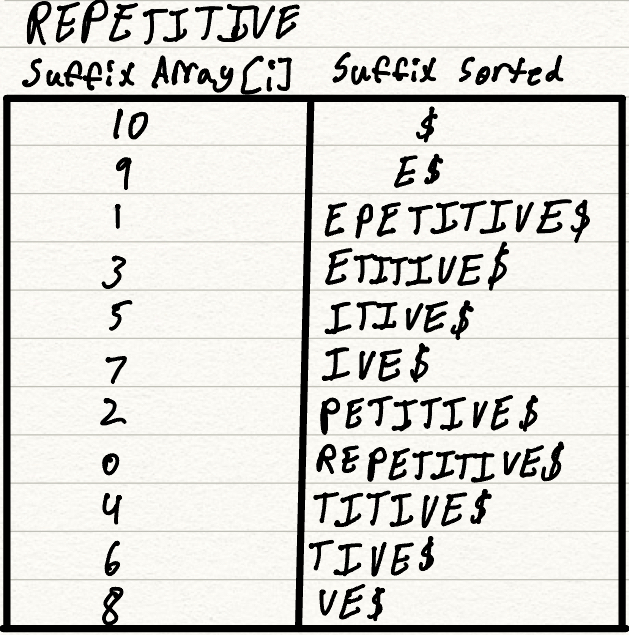
\includegraphics[scale=.4]{images/Suffix_array-1.jpeg}
    \item 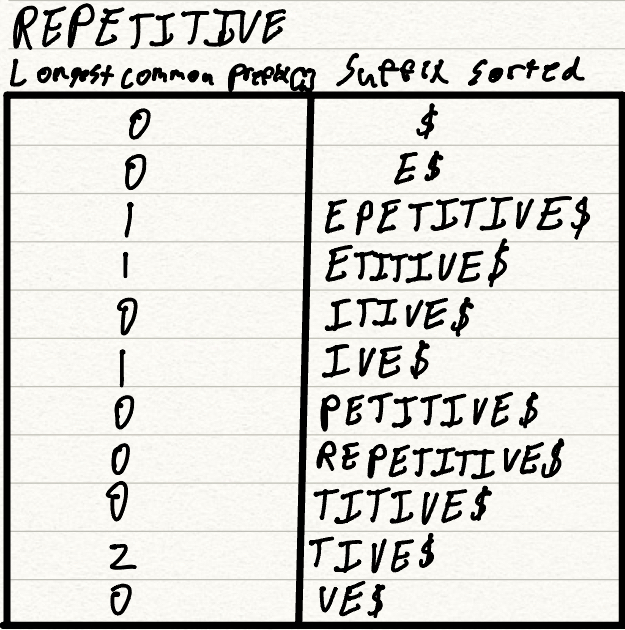
\includegraphics[scale=.4]{images/LCP-1.jpeg}
    \item To find all occurrences of a string $P$ in a larger string $S$ we would have to use suffix and LCP arrays built from $S$.
    We can do this by first building the suffix array for $S$ and then building the LCP array for $S$. 
    We then use binary search on the suffix array to find the index of the first occurrence and pattern of $P$ in $S$, getting us a pattern where $P$ occurs in $S$.
    We can then use the LCP array to find the number of occurrences of $P$ in $S$.
    Since the LCP array stores the length of the longest common prefix for each pair of adjacent strings, we can use this to find the number of occurrences of $P$ in $S$.
    We can do this by comparing the length of the longest common prefix of the suffixes at the current index and the next index, both backwards and forwards, to the length of $P$.
    If the length of the longest common prefix is greater than or equal to the length of $P$, we know that the suffixes at the current index and the next index have $P$ as a prefix.
    We can then increment the number of occurrences of $P$ in $S$ by 1 and continue to the next index.
    If the length of the longest common prefix is less than the length of $P$, we know that the suffixes at the current index and the next index do not have $P$ as a prefix.
    We can then stop the loop and return the number of occurrences of $P$ in $S$.
    \item We would prefer to use suffix arrays over suffix trees when the alphabet is large.
    This is because suffix arrays are easier to traverse than suffix trees.
    Suffix arrays are sorted lexographically so we can use binary search to quickly find a string in the suffix array.
    For suffix trees, we would have to traverse the whole tree to find a string therefore we would have to look at every suffix in tree.
    By having more efficient traversal, suffix arrays are better for large alphabets.
\end{enumerate}


\section*{Problem 3 -- Hashing (25\%)}
Consider the following simple hash function $h$ for mapping keys $z_j \in Z$ for $j=1,\dots ,n$ to array indices $\{1, \dots  m\}$.
For each key $z \in Z$, $h(z)=i$ with probability $1/m$ where $i=1, \dots , m$.
What is the expected number of keys such that $h(a)=h(b)$ over all keys $a \neq b$?
\textit{Hint: you want to define a similar random variable representing collisions as we did in Lecture 22 or Chapter 1.5 of the Algorithms textbook.}

We can let $X$ be the random variable for the number of collisions.
We can now have a indicator random variable $I$ where $I=1$ if there is a collision and $I=0$ if there is no collision
if a insertion of $b$ causes a collision.

We know that:\\ 
\begin{center}
$P(h(a) = h(b)) = \frac{1}{m}$\\
\end{center}
So we can define X as:\\
\begin{equation}
    X = \sum_{i=1}^{n} \sum_{j=i+1}^{n} X_{ij}
\end{equation}
We can now get the expected number of collisions by taking the expected value of X:\\
\begin{equation}
    E(X) = \sum_{i=1}^{n} \sum_{j=i+1}^{n} E(X_{ij}) = \sum_{i=1}^{n} \sum_{j=i+1}^{n} \frac{1}{m} = \frac{n(n-1)}{2m}
\end{equation}




\end{document}
